\mbox{$\displaystyle -\,$\,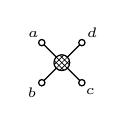
\begin{tikzpicture}[x=0.500cm, y=0.500cm, line width=0.450pt, baseline={([yshift=-0.6ex]0,0)}]
  \draw (-0.509,0.509) -- (0.000,0.000);
  \draw (-0.509,-0.509) -- (0.000,0.000);
  \draw (0.509,-0.509) -- (0.000,0.000);
  \draw (0.509,0.509) -- (0.000,0.000);
  \fill[white] (0.000,0.000) circle (0.200);
  \draw[line width=0.248pt] (-0.193,-0.052) -- (0.052,0.193) (-0.141,-0.141) -- (0.141,0.141) (-0.052,-0.193) -- (0.193,0.052) (-0.193,0.052) -- (0.052,-0.193) (-0.141,0.141) -- (0.141,-0.141) (-0.052,0.193) -- (0.193,-0.052);
  \draw (0.000,0.000) circle (0.200);
  \draw[fill=white] (-0.509,0.509) circle (0.080);
  \draw[fill=white] (-0.509,-0.509) circle (0.080);
  \draw[fill=white] (0.509,-0.509) circle (0.080);
  \draw[fill=white] (0.509,0.509) circle (0.080);
  \node[font=\tiny, inner sep=0pt, anchor=315] at (-0.629,0.629) {$a$};
  \node[font=\tiny, inner sep=0pt, anchor=45] at (-0.629,-0.629) {$b$};
  \node[font=\tiny, inner sep=0pt, anchor=135] at (0.629,-0.629) {$c$};
  \node[font=\tiny, inner sep=0pt, anchor=225] at (0.629,0.629) {$d$};
\end{tikzpicture}}
\diagramgap
\mbox{$\displaystyle +\,$\,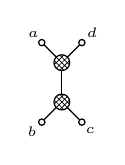
\begin{tikzpicture}[x=0.500cm, y=0.500cm, line width=0.450pt, baseline={([yshift=-0.6ex]0,0)}]
  \draw (-0.509,1.009) -- (0.000,0.500);
  \draw (-0.509,-1.009) -- (0.000,-0.500);
  \draw (0.509,-1.009) -- (0.000,-0.500);
  \draw (0.509,1.009) -- (0.000,0.500);
  \draw (0.000,0.500) -- (0.000,-0.500);
  \fill[white] (0.000,0.500) circle (0.200);
  \draw[line width=0.248pt] (-0.193,0.448) -- (0.052,0.693) (-0.141,0.359) -- (0.141,0.641) (-0.052,0.307) -- (0.193,0.552) (-0.193,0.552) -- (0.052,0.307) (-0.141,0.641) -- (0.141,0.359) (-0.052,0.693) -- (0.193,0.448);
  \draw (0.000,0.500) circle (0.200);
  \fill[white] (0.000,-0.500) circle (0.200);
  \draw[line width=0.248pt] (-0.193,-0.552) -- (0.052,-0.307) (-0.141,-0.641) -- (0.141,-0.359) (-0.052,-0.693) -- (0.193,-0.448) (-0.193,-0.448) -- (0.052,-0.693) (-0.141,-0.359) -- (0.141,-0.641) (-0.052,-0.307) -- (0.193,-0.552);
  \draw (0.000,-0.500) circle (0.200);
  \draw[fill=white] (-0.509,1.009) circle (0.080);
  \draw[fill=white] (-0.509,-1.009) circle (0.080);
  \draw[fill=white] (0.509,-1.009) circle (0.080);
  \draw[fill=white] (0.509,1.009) circle (0.080);
  \node[font=\tiny, inner sep=0pt, anchor=315] at (-0.629,1.129) {$a$};
  \node[font=\tiny, inner sep=0pt, anchor=45] at (-0.629,-1.129) {$b$};
  \node[font=\tiny, inner sep=0pt, anchor=135] at (0.629,-1.129) {$c$};
  \node[font=\tiny, inner sep=0pt, anchor=225] at (0.629,1.129) {$d$};
\end{tikzpicture}}
\diagramgap
\mbox{$\displaystyle +\,$\,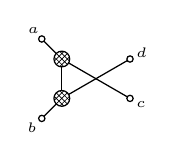
\begin{tikzpicture}[x=0.500cm, y=0.500cm, line width=0.450pt, baseline={([yshift=-0.6ex]0,0)}]
  \draw (-0.509,1.009) -- (0.000,0.500);
  \draw (-0.509,-1.009) -- (0.000,-0.500);
  \draw (1.732,-0.500) -- (0.000,0.500);
  \draw (1.732,0.500) -- (0.000,-0.500);
  \draw (0.000,0.500) -- (0.000,-0.500);
  \fill[white] (0.000,0.500) circle (0.200);
  \draw[line width=0.248pt] (-0.193,0.448) -- (0.052,0.693) (-0.141,0.359) -- (0.141,0.641) (-0.052,0.307) -- (0.193,0.552) (-0.193,0.552) -- (0.052,0.307) (-0.141,0.641) -- (0.141,0.359) (-0.052,0.693) -- (0.193,0.448);
  \draw (0.000,0.500) circle (0.200);
  \fill[white] (0.000,-0.500) circle (0.200);
  \draw[line width=0.248pt] (-0.193,-0.552) -- (0.052,-0.307) (-0.141,-0.641) -- (0.141,-0.359) (-0.052,-0.693) -- (0.193,-0.448) (-0.193,-0.448) -- (0.052,-0.693) (-0.141,-0.359) -- (0.141,-0.641) (-0.052,-0.307) -- (0.193,-0.552);
  \draw (0.000,-0.500) circle (0.200);
  \draw[fill=white] (-0.509,1.009) circle (0.080);
  \draw[fill=white] (-0.509,-1.009) circle (0.080);
  \draw[fill=white] (1.732,-0.500) circle (0.080);
  \draw[fill=white] (1.732,0.500) circle (0.080);
  \node[font=\tiny, inner sep=0pt, anchor=315] at (-0.629,1.129) {$a$};
  \node[font=\tiny, inner sep=0pt, anchor=45] at (-0.629,-1.129) {$b$};
  \node[font=\tiny, inner sep=0pt, anchor=150] at (1.879,-0.585) {$c$};
  \node[font=\tiny, inner sep=0pt, anchor=210] at (1.879,0.585) {$d$};
\end{tikzpicture}}
\diagramgap
\mbox{$\displaystyle +\,$\,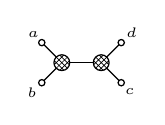
\begin{tikzpicture}[x=0.500cm, y=0.500cm, line width=0.450pt, baseline={([yshift=-0.6ex]0,0)}]
  \draw (-1.009,0.509) -- (-0.500,0.000);
  \draw (-1.009,-0.509) -- (-0.500,0.000);
  \draw (1.009,-0.509) -- (0.500,0.000);
  \draw (1.009,0.509) -- (0.500,0.000);
  \draw (-0.500,0.000) -- (0.500,0.000);
  \fill[white] (-0.500,0.000) circle (0.200);
  \draw[line width=0.248pt] (-0.693,-0.052) -- (-0.448,0.193) (-0.641,-0.141) -- (-0.359,0.141) (-0.552,-0.193) -- (-0.307,0.052) (-0.693,0.052) -- (-0.448,-0.193) (-0.641,0.141) -- (-0.359,-0.141) (-0.552,0.193) -- (-0.307,-0.052);
  \draw (-0.500,0.000) circle (0.200);
  \fill[white] (0.500,0.000) circle (0.200);
  \draw[line width=0.248pt] (0.307,-0.052) -- (0.552,0.193) (0.359,-0.141) -- (0.641,0.141) (0.448,-0.193) -- (0.693,0.052) (0.307,0.052) -- (0.552,-0.193) (0.359,0.141) -- (0.641,-0.141) (0.448,0.193) -- (0.693,-0.052);
  \draw (0.500,0.000) circle (0.200);
  \draw[fill=white] (-1.009,0.509) circle (0.080);
  \draw[fill=white] (-1.009,-0.509) circle (0.080);
  \draw[fill=white] (1.009,-0.509) circle (0.080);
  \draw[fill=white] (1.009,0.509) circle (0.080);
  \node[font=\tiny, inner sep=0pt, anchor=315] at (-1.129,0.629) {$a$};
  \node[font=\tiny, inner sep=0pt, anchor=45] at (-1.129,-0.629) {$b$};
  \node[font=\tiny, inner sep=0pt, anchor=135] at (1.129,-0.629) {$c$};
  \node[font=\tiny, inner sep=0pt, anchor=225] at (1.129,0.629) {$d$};
\end{tikzpicture}}
